\section{Cluster Interaction}

\begin{frame}
	\frametitle{Overview -- Cluster Interaction}
	\begin{itemize}
		\item{Connecting to a cluster @ UH}
			\begin{itemize}
			\item Login to the cluster
			\item Verify user permissions
			\end{itemize}
    {\semitransp[25]{\item User directories
		\item Transferring files
		\begin{itemize}{\semitransp[25]{
			\item Globus
		}}\end{itemize}
		\item Software
		\begin{itemize}{\semitransp[25]{
			\item Modules
			\item Acquiring software
			\item Compilers
			}}
		\end{itemize}
		\item Managing user jobs
		\begin{itemize}{\semitransp[25]{
			\item Job scheduler
			\item Using SLURM
			\item Partitions			
			\item Submitting jobs (Examples)
			}}
		\end{itemize}			
		}}
	\end{itemize}
\end{frame}

\subsection{Connecting to a cluster @ UH}
\begin{frame}
	\frametitle{Connecting to a cluster @ UH}
	\begin{description}[\setlength{\leftmargini}{0pt}]
	\item[] \begin{itemize}
		\item To connect to the cluster, an SSH client is required
		\item Linux and MacOS X, typically have a SSH client already installed
		\item Windows typically needs a 3rd party SSH client
		\item Suggested SSH clients for Windows include:
		\begin{itemize}
			\item \href{http://www.hawaii.edu/askus/685}{SSH Secure Shell}~(SSH 3.2.9)
			\item \href{http://www.chiark.greenend.org.uk/~sgtatham/putty/download.html}{Putty}
                        \item \href{http://mobaxterm.mobatek.net/}{MobaXterm}
		\end{itemize}
	\end{itemize}
	\item[] ~\\
	\item[] \begin{itemize}
		\item The {\craycs} has one active login node:
		\begin{itemize}
			\item uhhpc1.its.hawaii.edu
			%\item uhhpc2.its.hawaii.edu
		\end{itemize}
	\end{itemize}
	\end{description}
        ~\\~\\
	{\large Let's attempt to login!}
\end{frame}


\subsubsection{Login to the {\craycs}}
\begin{frame}
\frametitle{Login to the {\craycs}}
	\begin{center}\textbf{Windows}\end{center}
	\hrule~\\
	\begin{itemize}
		\item If SSH 3.2.9 installed (Lab PCs have it installed)
		\item Open the start menu, and type ``SSH'' and you should see a program called ``SSH Secure File Terminal Client''
		\item Click ``Quick Connect'' and enter the following information:
			\begin{itemize}
			\item[] \textbf{Host Name:} uhhpc1.its.hawaii.edu %--OR-- uhhpc2.its.hawaii.edu
			\item[] \textbf{User Name:} Your UH User name e.g., user99
			\item[] \textbf{Port:} 22
			\end{itemize}
		\item Press ``Connect''
		\item Enter your UH user password when prompted and press the return key
	\end{itemize}
\end{frame}


\begin{frame}
\frametitle{Login to the {\craycs}}
	\begin{center}\textbf{Mac \& Linux}\end{center}
	\hrule~\\
	\begin{itemize}
		\item Open a terminal window
		\item Enter one of the following:
		\begin{itemize}
			\item ssh $<$UH User name$>$@uhhpc1.its.hawaii.edu
%			\item ssh $<$UH User name$>$@uhhpc2.its.hawaii.edu
			\item \textbf{Example:} ssh user99@uhhpc1.its.hawaii.edu
		\end{itemize}
		\item Enter your UH user password when prompted and press the return key
	\end{itemize}
\end{frame}


\begin{frame}
\frametitle{On Initial Login~\ldots}
	Validate that all system permissions are correct for your user~\\
	\begin{enumerate}
		\item Test that you can list files in your home: `\textcolor{blue}{\texttt{ls -la}}'    
		\item Test making a file in your home: `\textcolor{blue}{\texttt{touch test.txt}}'    
		\item Go into \ctilde{}/lus: `\textcolor{blue}{\texttt{cd \ctilde{}/lus/}}'  
		\item Test making a file in your lus directory: `\textcolor{blue}{\texttt{touch test.txt}}'   
		\item Go into \ctilde{}/apps:  `\textcolor{blue}{\texttt{cd \ctilde{}/apps/}}'     
		\item Test making a file in your apps directory: `\textcolor{blue}{\texttt{touch test.txt}}'   
	\end{enumerate}
	\begin{alertblock}{Result}
		\begin{center}Did you get any errors?  Let us know if you did\end{center}
	\end{alertblock}
	\btVFill
	
	\small Notes:
		\begin{itemize}\tiny
		\item On login you are placed in /home/$<$username$>$/
		\item By default, \ctilde{} is equivalent to /home/$<$username$>$/
		\end{itemize}
\end{frame}


\begin{frame}
	\frametitle{Overview -- Cluster Interaction}
	\begin{itemize}
		\item {\semitransp[25]{Connecting to a cluster @ UH}}
			\begin{itemize}{\semitransp[25]{
			\item Login to the cluster
			\item Verify user permissions
			}}
			\end{itemize}
    \item User directories
		{\semitransp[25]{\item Transferring files
		\begin{itemize}{\semitransp[25]{
			\item Globus
		}}\end{itemize}
		\item Software
		\begin{itemize}{\semitransp[25]{
			\item Modules
			\item Acquiring software
			\item Compilers
			}}
		\end{itemize}
		\item Managing user jobs
		\begin{itemize}{\semitransp[25]{
			\item Job scheduler
			\item Using SLURM
			\item Partitions			
			\item Submitting jobs (Examples)
			}}
		\end{itemize}			
		}}
	\end{itemize}
\end{frame}

\subsection{User Directories}
\begin{frame}[fragile]
\frametitle{User Directories}
\begin{block}{Home}
\begin{semiverbatim}\tiny \texttt
[user99@login \ctilde]\$ ls -l 
total 0
lrwxrwxrwx 1 user99 user99 23 Jan 15 20:38 \textcolor{teal}{apps} -> /lus/scratch/usr/user99
lrwxrwxrwx 1 user99 user99 19 Jan 15 20:38 \textcolor{teal}{lus} -> /lus/scratch/user99

\end{semiverbatim}
\end{block}
% lrwxrwxrwx 1 root   root   37 Jan 15 20:41 \colorbox{black}{\textcolor{red}{purge}} -> /lus/scratch/log/purge/current/user99
\begin{itemize}\footnotesize
		\item \ctilde{}/ is not on the {\lustre} filesystem and \textbf{should not be used for job data!}
		\item \ctilde{}/lus/ is a symlink to the {\lustre} scratch
		\begin{itemize}\tiny
			\item This is where all your job data files should live
			\item Items in this directory \emph{\textbf{are}} subject to our purge policy
		\end{itemize}
		\item \ctilde{}/apps/ is a symlink to where programs should be stored
		\begin{itemize}\tiny
			\item Items in this directory \emph{\textbf{are not}} subject to our purge policy
			\item Directory is monitored for abuse
		\end{itemize}
	\end{itemize}
\end{frame}


\begin{frame}[fragile]
\frametitle{User Directories}
\begin{block}{Filesystems}
\begin{semiverbatim}\tiny \texttt
[user99@login \ctilde]\$ df -h
Filesystem                                  Size  Used Avail Use% Mounted on
10.10.0.3:/ha_cluster/home                  1.8T  888G  851G  52% /home
10.12.0.51@o2ib:10.12.0.52@o2ib:/scratch    582T  429T  125T  78% /lus/scratch
\end{semiverbatim}
\end{block}
	\begin{itemize}\footnotesize
		\item /home/$<$username$>$ exists on a NFS mounted filesystem
		\begin{itemize}\tiny
			\item Only has 1.8TB of useable space
			\item Using all this space may cause problems for the entire cluster
			\item Not a high performance filesystem and small in size
		\end{itemize}
		\item /lus/scratch/ is the {\lustre} filesystem
		\begin{itemize}\tiny
			\item Has 582TB of useable space
			\item \ctilde{}/apps/ and \ctilde{}/lus/ point to directories on this filesystem
			\item High performance and a lot more space for users to use
			\item No hard or soft quotas are in place
			\item Utilization is managed through the  purge policy
		\end{itemize}
	\end{itemize}
\end{frame}


\begin{frame}
	\frametitle{Overview -- Cluster Interaction}
	\begin{itemize}
		\item {\semitransp[25]{Connecting to a cluster @ UH}}
			\begin{itemize}{\semitransp[25]{
			\item Login to the cluster
			\item Verify user permissions
			}}
			\end{itemize}
    {\semitransp[25]{\item User directories}}
		\item Transferring files
		\begin{itemize}
			\item Globus
		\end{itemize}
		{\semitransp[25]{
		\item Software
		\begin{itemize}{\semitransp[25]{
			\item Modules
			\item Acquiring software
			\item Compilers
			}}
		\end{itemize}
		\item Managing user jobs
		\begin{itemize}{\semitransp[25]{
			\item Job scheduler
			\item Using SLURM
			\item Partitions			
			\item Submitting jobs (Examples)
			}}
		\end{itemize}			
		}}
	\end{itemize}
\end{frame}


\subsection{Transferring Files}
\begin{frame}
	\frametitle{Available File Transfer Protocols}
	\begin{itemize}
		\item The cluster has the following options for transferring files:
		\begin{itemize}
			\item[--] scp (RCP$+$SSH protocol)
			\item[--] rsync (rsync protocol with SSH transport)
			\item[--] SFTP (SSH FTP protocol) -- Filezilla, Cyberduck
			\item[--] \href{https://www.globus.org/}{Globus} (Grid FTP protocol)
		\end{itemize}
		\item All options are widely used, and have clients that can be found for on most major operating systems
%               \item Please see the the CI website for links to several different clients?                 
	\end{itemize}
	\btVFill
	\begin{center}
		SFTP, scp, and rsync are fairly common on Linux systems,~\\but Globus is not as common~\ldots
	\end{center}
	
\end{frame}


\subsection{Globus}
\begin{frame}
	\frametitle{Globus}
	\begin{block}{What is Globus?}\footnotesize
	The Globus transfer service provides high-performance, secure, file transfer and synchronization between endpoints.~\\~\\
	Globus handles all the difficult aspects of data transfer, allowing application users to easily start and manage transfers between endpoints, while automatically tuning parameters to maximize bandwidth usage, managing security configurations, providing automatic fault recovery, and notifying users of completion and problems. 
	\end{block}
	\begin{definition}\tiny
	An \textbf{\emph{endpoint}} is one of the two file transfer locations -- either the source or the destination -- between which files can move.~\\Once a resource (such as a server, cluster, storage system, laptop, or other system) is defined as an endpoint, it will be available to authorized users who can transfer files to or from this endpoint.
	\end{definition}
{\tiny Please visit the {\ci} Globus quick start guide for instructions on how to use Globus:~\href{http://go.hawaii.edu/jMW}{http://go.hawaii.edu/jMW}}

        \numlessfootnotetxt{\tiny \url{https://www.globus.org/file-transfer}}
\end{frame}



%% \begin{frame}
%% 	\frametitle{Globus}\footnotesize
%% \begin{block}{How do I get Globus?}
%% To utilize Globus, follow the following steps:
%% \begin{itemize}\tiny
%% \item Register for a Globus Online account -- \url{https://www.globusonline.org/signup}
%% \item Sign in to Globus Online (using your Globus Online username and password) -- \url{https://www.globusonline.org/signin}
%% \item Select ‘Start Transfer’ under ‘File Transfer’, or from the drop down menu in the top bar
%% \item You can view the list of available endpoints by clicking the button on the ‘Endpoint’ drop down box
%% \begin{itemize}\tiny
%%  \item Each of the login nodes is also an endpoint: \textbf{\emph{UH-HPC1}} \& \textbf{\emph{UH-HPC2}}
%% \end{itemize}
%% \item Once you select an endpoint, a login window will pop up. You can access the UHHPC endpoints by simply using your UH username and password. Enter your UH accounts username in the ‘Username’ field and UH accounts password in the ‘Password’ field and click ‘Authenticate’. 
%% \item You will see a listing of the contents of your home directory on the UH HPC. Double click on a directory to view its contents
%% \item Select a file or directory and click on the highlighted ‘arrow button’ to initiate the transfer
%% \end{itemize}
%% \end{block}
%% ~\\
%% \end{frame}


%% \begin{frame}
%% 	\frametitle{Globus}
%%         \begin{itemize}
%%           \item In order to transfer data from the {\craycs} to your personal computer, a client called the Globus Connect Personal (\url{https://www.globus.org/globus-connect-personal}) needs to be installed
%%           \item The Globus Connect Personal, turns your personal computer into a private endpoint that is only useable with your personal Globus Online account.
%%           \item If you want to install Globus on your own server, Globus Connect (\url{https://www.globus.org/globus-connect-server}) is required
%%             \item If issues arise while trying to install Globus Connect or Globus Connect Personal,  please contact us and we will be more than happy to help
%% \end{itemize} 
%% \end{frame}

\begin{frame}
	\frametitle{Overview -- Cluster Interaction}
	\begin{itemize}
		\item {\semitransp[25]{Connecting to a cluster @ UH}}
			\begin{itemize}{\semitransp[25]{
			\item Login to the cluster
			\item Verify user permissions
			}}
			\end{itemize}
   {\semitransp[25]{ \item User directories
		\item Transferring files
		\begin{itemize}{\semitransp[25]{
			\item Globus
		}}\end{itemize}
		}}
		\item Software
		\begin{itemize}
			\item Modules
			\item Acquiring software
			\item Compilers
		\end{itemize}
		{\semitransp[25]{
		\item Managing user jobs
		\begin{itemize}{\semitransp[25]{
			\item Job scheduler
			\item Using SLURM
			\item Partitions
			\item Submitting jobs (Examples)
			}}
		\end{itemize}			
		}}
	\end{itemize}
\end{frame}


\subsection{Software}
\begin{frame}
	\frametitle{Modules}
	\begin{block}{Modules}\tiny
	  A tool to help users manage their Unix or Linux shell environment, by allowing groups of related environment-variable settings to be made or removed dynamically.\footnote{\label{wiki_module}\tiny\
             \url{https://en.wikipedia.org/wiki/Environment_Modules_(software)}}
	
	\end{block}
	\begin{itemize}
		\item We globally install frequently requested software packages and create modules for all users to access
		\item Access to modules is via the \textbf{module} command
		\begin{itemize}\footnotesize
			\item `module avail' -- list installed modules
			\item `module show $<$module name$>$' -- Show what actions a module performs
			\item `module load $<$module name$>$' -- Loads the named module
                        \item `module list -- Show what modules are loaded
			\item `module purge' -- Unload all loaded modules
		\end{itemize}
		\item Installing software in your \ctilde{}/apps directory is suggested to prevent us from being a bottleneck
	\end{itemize}

\end{frame}


\begin{frame}
	\frametitle{Acquiring Software -- Binaries and/or Source}
	\begin{itemize}
		\item	You can transfer software source, binaries or scripts into your \ctilde{}/apps directory on the {\craycs}
		\begin{itemize}
			\item Binaries compiled as x86\_64 (64-bit) for CentOS 6.5 or RHEL6.5 should work
		\end{itemize}
		\item You may also download tar or zipped software/source code directly from the login nodes using tools like \textbf{wget} \& \textbf{curl}
		\item You may also clone source repositories using the correct software revision tool: \textbf{git}, \textbf{svn}, \textbf{hg}, \textbf{cvs}, etc.
	\end{itemize}
\end{frame}


\begin{frame}
\frametitle{Compilers}
	\begin{itemize}
		\item We have the {\intel} \& GNU (gcc, g$++$) compilers
		\item Compiling must take place on a compute node
		\begin{itemize}
			\item Interactive sessions are useful for compiling software
			\item Sandbox nodes mirror the environment the compute nodes provide and are ideal for compilation
			\item Login nodes \textbf{do not} mirror the compute node environment
		\end{itemize}
		\item {\intel} compilers are recommended for best performance
		\begin{itemize}
			\item {\intel} 2013 compilers:
			\begin{itemize}
				\item module load intel/ics -- Loads {\intel} compilers: {\tiny \textbf{icc}, \textbf{ifort}, \textbf{icpc}}
				\item module load intel/impi -- Loads {\intel} MPI wrapper: {\tiny\textbf{mpiicc}, \textbf{mpiifort}, \textbf{mpiicpc}}
			\end{itemize}
			\item {\intel} 2016 compilers:
			\begin{itemize}
				\item We have 2 floating seats for {\intel} 2016 compiler
				\item intel\_2016/ics 
				\item intel\_2016/impi 
			\end{itemize}
		\end{itemize}			
	\end{itemize}
\end{frame}


\begin{frame}
	\frametitle{Overview -- Cluster Interaction}
	\begin{itemize}
		\item {\semitransp[25]{Connecting to a cluster @ UH}}
			\begin{itemize}{\semitransp[25]{
			\item Login to the cluster
			\item Verify user permissions
			}}
			\end{itemize}
   {\semitransp[25]{ \item User directories
		\item Transferring files
		\begin{itemize}{\semitransp[25]{
			\item Globus
		}}\end{itemize}
		\item Software
		\begin{itemize}{\semitransp[25]{
			\item Modules
			\item Acquiring software
			\item Compilers
			}}
		\end{itemize}
		}}
		\item Managing user jobs
		\begin{itemize}
			\item Job scheduler
			\item Using SLURM
			\item Partitions
			\item Submitting jobs (Examples)
		\end{itemize}		
	\end{itemize}
\end{frame}


\subsection{Managing User Jobs}
\begin{frame}
\frametitle{Managing User Jobs}
User jobs all come in different shapes and sizes:  
\begin{itemize}\footnotesize
	\item Require multiple nodes working in concert towards a common goal (MPI)
	\item Require a single node, in which they use multiple threads~\\work together (OpenMP, pthreads)
	\item Require a lot of cores to process a lot of data in an identical manner,~\\yet none of the inputs have dependencies on another (HTC)
\end{itemize}
\bigskip
The {\craycs} is capable of handling many different types of jobs, but with so many users in a multi-user environment, how do we impose order on this chaos?
\btVFill
\begin{center}This looks like a job for a \textbf{\emph{job scheduler}}!\end{center}
\end{frame}

\begin{frame}
  \frametitle{Job Schedulers}
  \begin{block}{Purpose}To control and prioritize the execution order of unrelated jobs\end{block}
	Basic features expected of a job scheduler:
	\begin{itemize}\footnotesize
        \item Provides a user interface for users to request resources and monitor work 
        \item Allocates access to resources for the requested duration of time
	\item Starts, monitors and terminates work on allocated resources
	\item Arbitrates contention for resources by managing queues of pending work
	\end{itemize}
	\bigskip
        The {\craycs} uses the \textbf{S}imple \textbf{L}inux \textbf{U}tility for \textbf{R}esource \textbf{M}anagement~\\ or simply known as the \emph{SLURM scheduler}
	\numlessfootnotetxt{\tiny \url{https://en.wikipedia.org/wiki/Slurm_Workload_Manager}}
	\numlessfootnotetxt{\tiny \url{http://slurm.schedmd.com/slurm.html}}
\end{frame}

\subsection{SLURM}
\begin{frame}
\frametitle{SLURM}
\begin{block}{How are jobs scheduled?}
User submitted jobs are assigned a priority using a fairshare algorithm.\\
Factors such as the following are all used to assign a priority to a given job: 
\begin{itemize}
\item Runtime
\item Amount of resources requested
\item Age of job
\item Amount of core hours a user has used in recent history
\end{itemize}

\end{block}
\end{frame}

\begin{frame}
\frametitle{SLURM commands}\footnotesize
SLURM has a series of commands, each of which allow users to interact with the job scheduler
\begin{itemize}\tiny
	\item \emph{\textbf{srun}} --  Used to submit a job for execution or initiate job steps in real time
	\item \emph{\textbf{sbatch}} -- Used to submit a job script for later execution. The script could contain one or more srun commands
	\item \emph{\textbf{squeue}} -- Reports the state of jobs or job steps
	\item \emph{\textbf{scancel}} -- Used to cancel a pending or running job or job step. It can also be used to send an arbitrary signal to all processes associated with a running job or job step
	\item \emph{\textbf{sinfo}} -- Reports the state of partitions and nodes managed by Slurm. It has a wide variety of filtering, sorting, and formatting options
	\item \emph{\textbf{sacct}} -- Used to report job or job step accounting information about active or completed jobs
	\item \emph{\textbf{scontrol}} -- The administrative tool used to view and/or modify Slurm state. Note that many scontrol commands can only be executed as user root
\end{itemize}
\begin{itemize}
	\item[--] Examples usage of the SLURM commands can be seen on schedmd's \href{http://slurm.schedmd.com/quickstart.html}{quickstart}
	\item[--] Each command should have a `man' page, or displays help when the -h flag is used
\end{itemize}
\numlessfootnotetxt{\tiny \url{http://slurm.schedmd.com/quickstart.html}}
\end{frame}


\subsection{SLURM Partitions}
\begin{frame}
\footnotesize
\frametitle{Partitions}
\begin{block}{What is a partition?}\footnotesize
A partition can be thought of as a group of nodes/resources divided into possibly overlapping sets.  Each partition can be considered as a job queue, each of which has an assortment of constraints such as job size limit, job time limit, users permitted to use it, etc. Priority-ordered jobs are allocated nodes within a partition until the resources (nodes, processors, memory, etc.) within that partition are exhausted.\footnote{\label{schedmd_qstart}\tiny \url{http://slurm.schedmd.com/quickstart.html}}
\end{block}
\begin{itemize}
	\item The current public partitions on the {\craycs}:~\\\textbf{community.q}, \textbf{exclusive.q}, \textbf{lm.q}, \textbf{gpu.q}, \textbf{sb.q}, \textbf{kill.q}, \textbf{kill.gpu.q}, \textbf{htc.q}
	\item Jobs submitted to kill.q and htc.q can be preempted by jobs in other partitions
\end{itemize}
\end{frame}

\begin{frame}
\frametitle{Partitions}
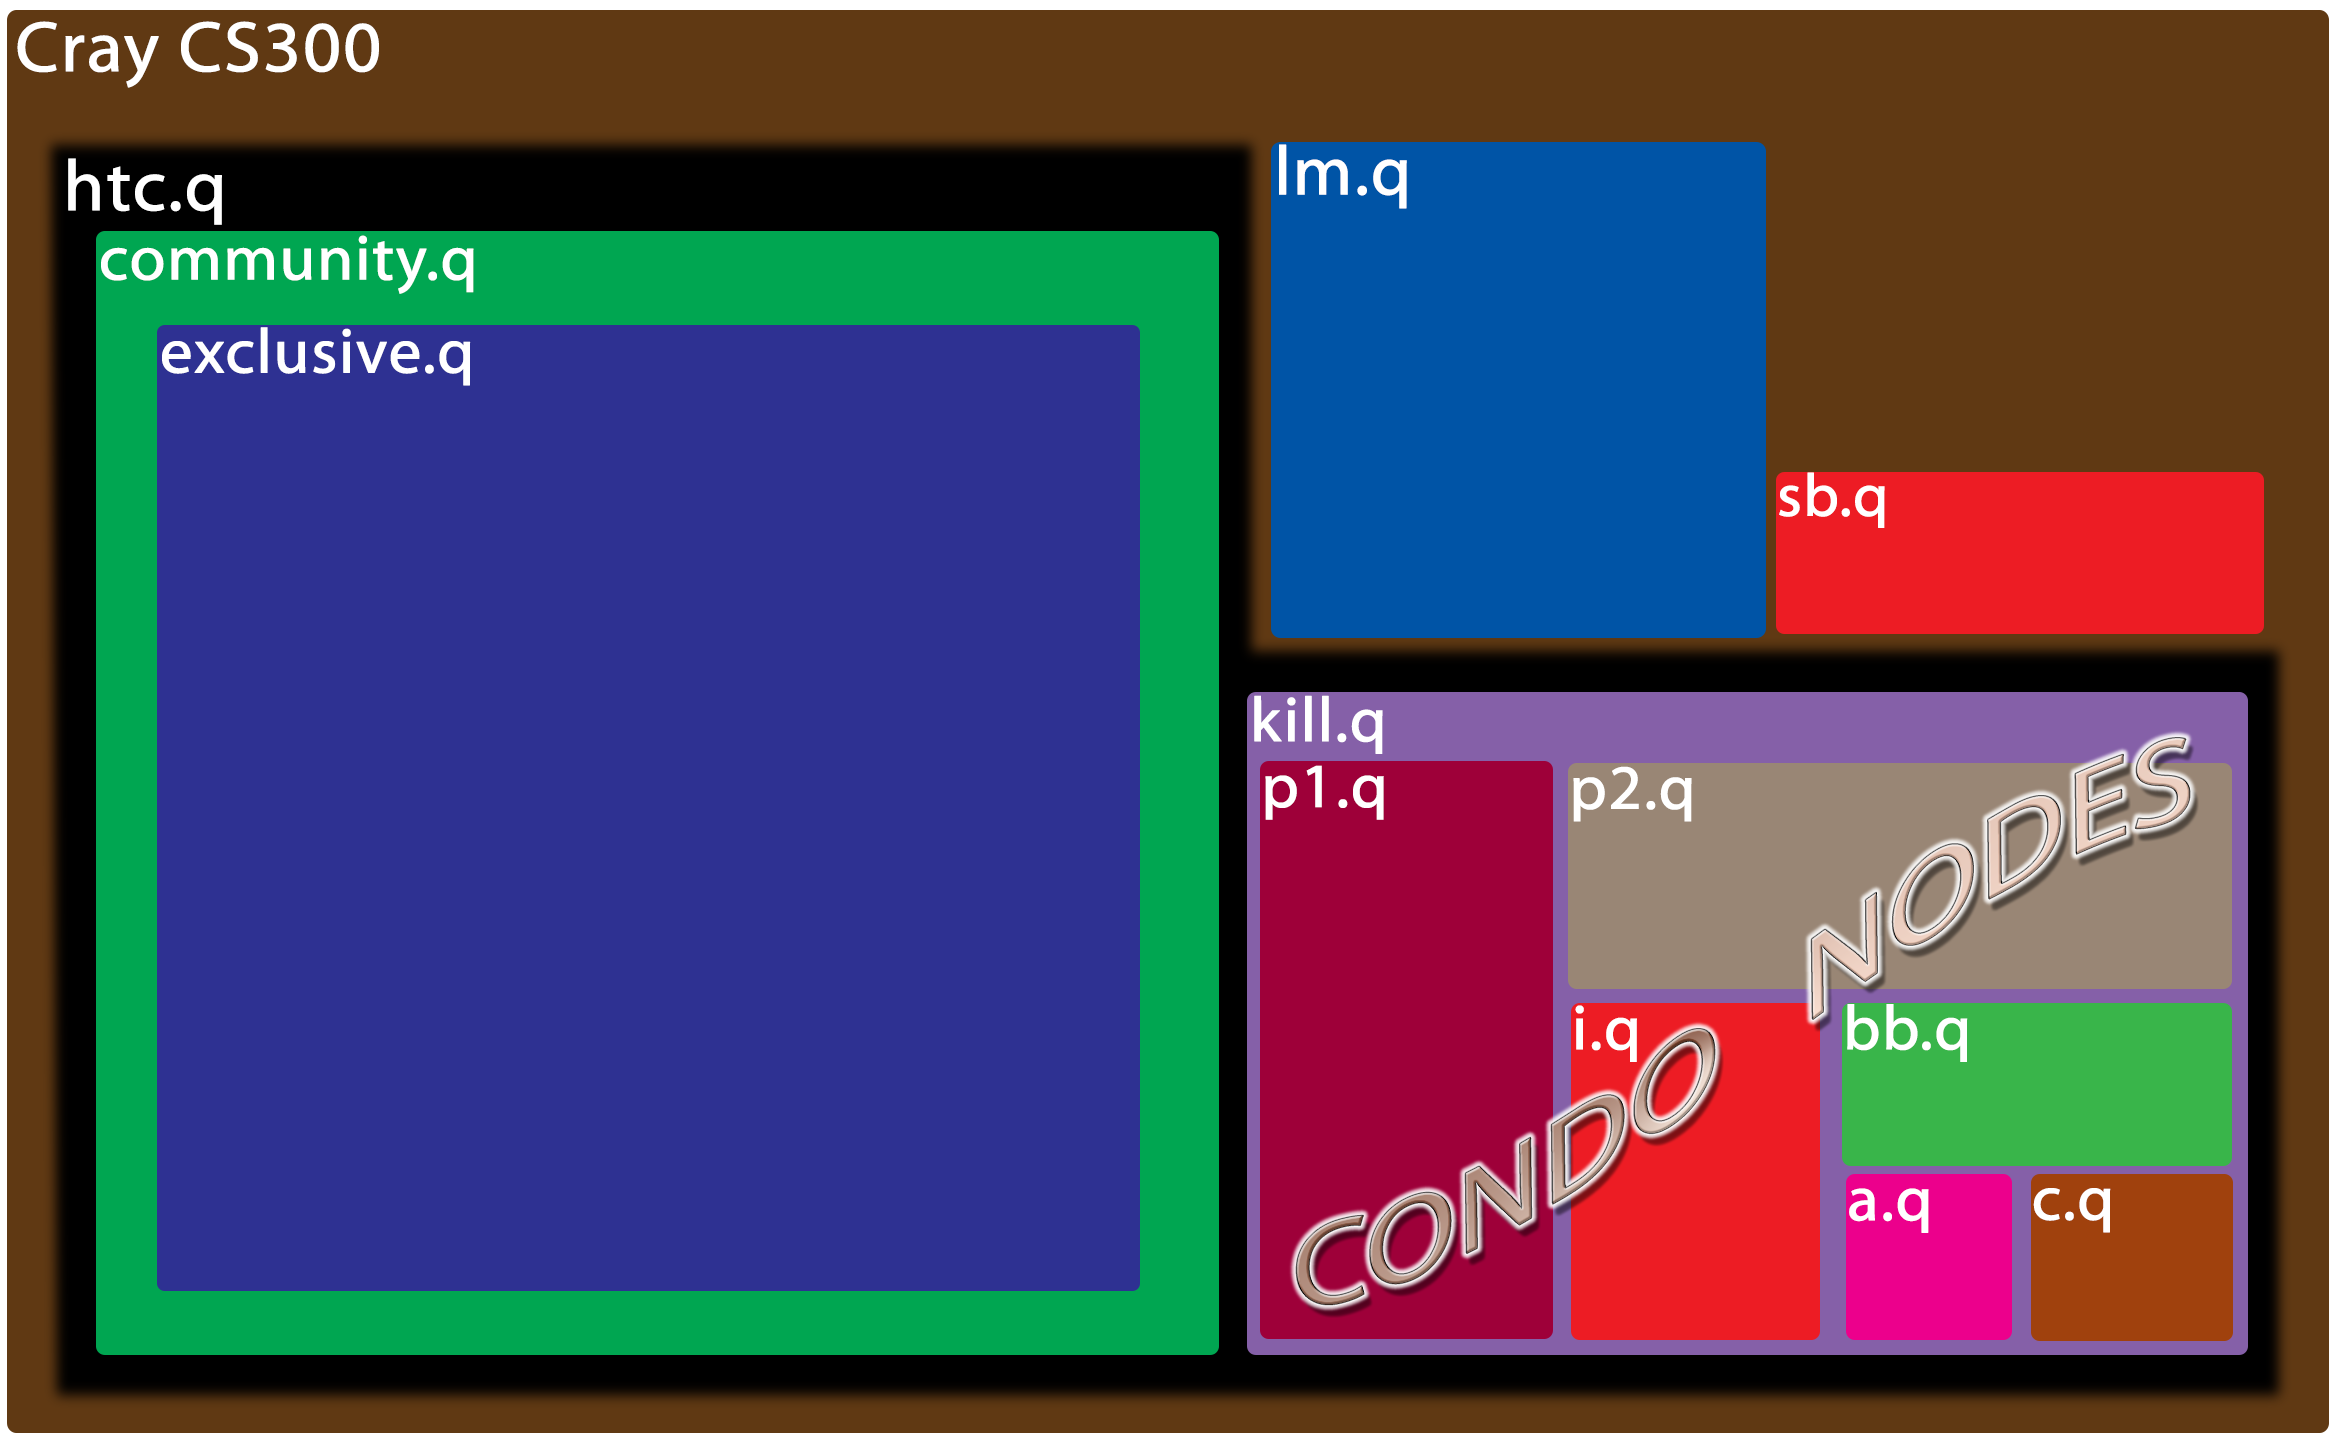
\includegraphics[width=0.95\textwidth]{images/partitions}
\end{frame}

\begin{frame}
\frametitle{Partition Details}
\resizebox{0.95\textwidth}{!}{%
\begin{tabular}{l || c || c || c || c || c || c}
\toprule                                                                    
\textbf{Partition} & \textbf{Time} & \textbf{Nodes per job} & \textbf{Priority} & \textbf{Shared} & \textbf{Preempt Mode} & \textbf{Memory per CPU (MB)} \\
%\toprule                                                                    
%\toprule                                                                    
\midrule
\midrule
community.q & \begin{tabular}{l r} \textbf{Default:} & 0-00:10:00~\\ \textbf{Max:} & 3-00:00:00\end{tabular} & \begin{tabular}{c c} \textbf{Min:} & \padfrom{\ \ \ }{1}~\\ \textbf{Max:} & \padfrom{\ \ \ }{1}\end{tabular} & 10 & NO & OFF & \begin{tabular}{l c}\textbf{Default:} & \padfrom{\ \ \ \ \ \ \ }{3250}~\\ \textbf{Max:} & \padfrom{\ \ \ \ \ \ \ \ }{$\infty$}\end{tabular}\\
\hline
\hline
exclusive.q & \begin{tabular}{l r}\textbf{Default:} & 0-00:10:00~\\ \textbf{Max:} & 3-00:00:00\end{tabular} &  \begin{tabular}{c  c}\textbf{Min:}& \padfrom{\ \ \ }{1}~\\ \textbf{Max:}&\padfrom{\ \ \ }{20}\end{tabular} & 10 & EXCLUSIVE & OFF & \begin{tabular}{l c}\textbf{Default:} & \padfrom{\ \ \ \ \ \ \ \ }{$\infty$}~\\ \textbf{Max:} & \padfrom{\ \ \ \ \ \ \ \ }{$\infty$}\end{tabular}\\
\hline
\hline
gpu.q & \begin{tabular}{l r} \textbf{Default:} & 0-00:10:00~\\ \textbf{Max:} & 3-00:00:00\end{tabular} & \begin{tabular}{c c} \textbf{Min:} & \padfrom{\ \ \ }{1}~\\ \textbf{Max:} & \padfrom{\ \ \ }{1}\end{tabular} & 10 & NO & OFF & \begin{tabular}{l c}\textbf{Default:} & \padfrom{\ \ \ \ \ \ \ }{3250}~\\ \textbf{Max:} & \padfrom{\ \ \ \ \ \ \ \ }{$\infty$}\end{tabular}\\
\hline
\hline
kill.q & \begin{tabular}{l r}\textbf{Default:} & 0-00:10:00~\\ \textbf{Max:} & 3-00:00:00\end{tabular} &  \begin{tabular}{c  c}\textbf{Min:} & \padfrom{\ \ \ }{1}~\\ \textbf{Max:} &\padfrom{\ \ \ }{20}\end{tabular} & 10 & NO & REQUEUE & \begin{tabular}{l c}\textbf{Default:} & \padfrom{\ \ \ \ \ \ \ }{3250}~\\ \textbf{Max:} & \padfrom{\ \ \ \ \ \ \ \ }{$\infty$}\end{tabular}\\
\hline
\hline
kill.gpu.q & \begin{tabular}{l r}\textbf{Default:} & 0-00:10:00~\\ \textbf{Max:} & 3-00:00:00\end{tabular} &  \begin{tabular}{c  c}\textbf{Min:} & \padfrom{\ \ \ }{1}~\\ \textbf{Max:} &\padfrom{\ \ \ }{1}\end{tabular} & 10 & NO & REQUEUE & \begin{tabular}{l c}\textbf{Default:} & \padfrom{\ \ \ \ \ \ \ }{3250}~\\ \textbf{Max:} & \padfrom{\ \ \ \ \ \ \ \ }{$\infty$}\end{tabular}\\
\hline
\hline
htc.q & \begin{tabular}{l r}\textbf{Default:} & 0-00:10:00~\\ \textbf{Max:} & 3-00:00:00\end{tabular} &  \begin{tabular}{c  c}\textbf{Min:} & \padfrom{\ \ \ }{1}~\\ \textbf{Max:} &\padfrom{\ \ \ }{1}\end{tabular} & 1 & NO & REQUEUE & \begin{tabular}{l c}\textbf{Default:} & \padfrom{\ \ \ \ \ \ \ }{3250}~\\ \textbf{Max:} & \padfrom{\ \ \ \ \ \ \ \ }{$\infty$}\end{tabular}\\
\hline
\hline
lm.q & \begin{tabular}{l r}\textbf{Default:} & 0-00:10:00~\\ \textbf{Max:} & 3-00:00:00\end{tabular} &  \begin{tabular}{c  c}\textbf{Min:} & \padfrom{\ \ \ }{1}~\\ \textbf{Max:} &\padfrom{\ \ \ }{1}\end{tabular} & 10 & NO & OFF & \begin{tabular}{l c}\textbf{Default:} & \padfrom{\ \ \ \ \ \ \ \ }{$\infty$}~\\ \textbf{Max:} & \padfrom{\ \ \ \ \ \ \ \ }{$\infty$}\end{tabular}\\
\hline
\hline
sb.q & \begin{tabular}{l r}\textbf{Default:} & 0-00:05:00~\\ \textbf{Max:} & 0-01:00:00\end{tabular} &  \begin{tabular}{c  c}\textbf{Min:} & \padfrom{\ \ \ }{1}~\\ \textbf{Max:} &\padfrom{\ \ \ }{2}\end{tabular} & 10 & NO & OFF & \begin{tabular}{l c}\textbf{Default:} & \padfrom{\ \ \ \ \ \ \ }{3250}~\\ \textbf{Max:} & \padfrom{\ \ \ \ \ \ \ \ }{$\infty$}\end{tabular}\\
\bottomrule 
\end{tabular}   
}
\\
\bigskip
Partition details also available on the \href{http://www.hawaii.edu/its/ci/hpc-resources/slurm-partitions/}{{\ci} website} or by using the following command:
\\
\texttt{$[$login \ctilde$]$\$ scontrol show partition $<$partition name$>$}
\end{frame}

\subsection{Interactive Job -- srun}
\frametitle{SLURM Job Scripts}
\begin{frame}
  \frametitle{Interactive Job with SLURM}
  \begin{block}{Interactive session}\tiny
    $[$login \ctilde$]$\$ srun \ddash{}immediate \ddash{}partition sb.q \ddash{}nodes 1 \ddash{}cpus-per-task 1 \ddash{}tasks-per-node 1 \ddash{}time 0-01:00:00 \ddash{}pty /bin/bash
    ~\\
    ~\\
    ~\\
    \hrule\begin{semiverbatim}$[$login \ctilde$]$\$ srun -I -p sb.q -N 1 -c 1 -n 1 -t 0-01:00:00 \ddash{}pty /bin/bash\end{semiverbatim}

  \end{block}
  \btVFill
  \begin{center}Interactive sessions terminate when the specified time has elapsed~\\or if you give the \textbf{exit} command \end{center}

  \end{frame}



\subsection{GPU Batch Job Example Script}
\begin{frame}[fragile]
\frametitle{SLURM sbatch -- Submission Script File -- GPU}
\begin{semiverbatim}\tiny
[login lus]\$ cat gpu.slurm

\#!/bin/bash
\#SBATCH \ddash{}job-name=GPU\_example
\textcolor{blue}{\#SBATCH \ddash{}partition=gpu.q}
\#SBATCH \ddash{}time=3-00:00:00 ## time format is DD-HH:MM:SS
\#\# task-per-node x cpus-per-task should not typically exceed core count on an individual node 
\#SBATCH \ddash{}nodes=1
\#SBATCH \ddash{}tasks-per-node=1
\textcolor{blue}{\#SBATCH \ddash{}cpus-per-task=10}
\textcolor{blue}{\#SBATCH \ddash{}mem=11000} \#\# max amount of memory per node you require
\textcolor{blue}{\#SBATCH \ddash{}gres=gpu:NV-K40:2 } \#\# request both GPUs in the GPU node
\#\#\# To request only 1 of the two GPUs in the node, you would do: gpu:NV-K40:1
\#SBATCH \ddash{}error=hello-\%A.err \#\# \%A - filled with jobid
\#SBATCH \ddash{}output=hello-\%A.out \#\# \%A - filled with jobid
\#\# Useful for remote notification
\#SBATCH \ddash{}mail-type=BEGIN,END,FAIL,REQUEUE,TIME\_LIMIT\_80
\#SBATCH \ddash{}mail-user=user@test.org

source \ctilde/.bash_profile \#if you want to use modules or need environment variables, source your bash profile
module load GPGPU/cuda/samples/7.5

\#\# All options and environment variables found on schedMD site: \href{http://slurm.schedmd.com/sbatch.html}{http://slurm.schedmd.com/sbatch.html}
export OMP\_NUM\_THREADS=\$\{SLURM\_CPUS\_PER\_TASK\}

bandwidthTest; cudaOpenMP; deviceQuery; simpleMultiGPU
\end{semiverbatim}
\end{frame}


\subsection{MPI Batch Job Example Script}
\begin{frame}[fragile]
\frametitle{SLURM sbatch -- Submission Script File (MPI Job)}
\begin{semiverbatim}\tiny
[login lus]\$ cat mpi.slurm

\#!/bin/bash
\#SBATCH \ddash{}job-name=MPI\_example
\textcolor{blue}{\#SBATCH \ddash{}partition=exclusive.q}
\#\# 3 day max run time for community.q, kill.q, exclusive.q, and htc.q.  1 Hour max run time for sb.q
\#SBATCH \ddash{}time=3-00:00:00 ## time format is DD-HH:MM:SS
\#\# task-per-node x cpus-per-task should not typically exceed core count on an individual node 
\textcolor{blue}{\#SBATCH \ddash{}nodes=4}
\textcolor{blue}{\#SBATCH \ddash{}tasks-per-node=20}
\textcolor{blue}{\#SBATCH \ddash{}cpus-per-task=1}
\textcolor{blue}{\#\#SBATCH \ddash{}mem=11000} \# Memory should not be set for jobs in exclusive.q
\#SBATCH \ddash{}error=hello-\%A.err \#\# \%A - filled with jobid
\#SBATCH \ddash{}output=hello-\%A.out \#\# \%A - filled with jobid
\#\# Useful for remote notification
\#SBATCH \ddash{}mail-type=BEGIN,END,FAIL,REQUEUE,TIME\_LIMIT\_80
\#SBATCH \ddash{}mail-user=user@test.org

source \ctilde/.bash_profile \#if you want to use modules or need environment variables, source your bash profile

\#\# All options and environment variables found on schedMD site: \href{http://slurm.schedmd.com/sbatch.html}{http://slurm.schedmd.com/sbatch.html}
\#\# Intel MPI manual: \href{https://software.intel.com/en-us/mpi-refman-lin-html}{https://software.intel.com/en-us/mpi-refman-lin-html}
export OMP\_NUM\_THREADS=\$\{SLURM\_CPUS\_PER\_TASK\}
export I\_MPI\_FABRICS=shm:tmi  
export I\_MPI\_PMI\_LIBRARY=/opt/local/slurm/default/lib64/libpmi.so

srun  -n \$\{SLURM\_NTASKS\}  ./hello\_mpi.intel 
\end{semiverbatim}
\end{frame}


\subsection{Non-MPI Batch Job Example Script}
\begin{frame}[fragile]
\frametitle{SLURM sbatch -- Submission Script File (Non-MPI Job)}
\begin{semiverbatim}\tiny
[login lus]\$ cat hello_world.slurm

\#!/bin/bash
\#SBATCH \ddash{}job-name=example
\textcolor{blue}{\#SBATCH \ddash{}partition=community.q}
\#\# 3 day max run time for community.q, kill.q, exclusive.q, and htc.q.  1 Hour max run time for sb.q
\#SBATCH \ddash{}time=3-00:00:00 ## time format is DD-HH:MM:SS
\#\# task-per-node x cpus-per-task should not typically exceed core count on an individual node 
\#SBATCH \ddash{}nodes=1
\#SBATCH \ddash{}tasks-per-node=1
\textcolor{blue}{\#SBATCH \ddash{}cpus-per-task=5}
\textcolor{blue}{\#SBATCH \ddash{}mem=11000} \#\# max amount of memory per node you require
\#SBATCH \ddash{}error=hello-\%A.err \#\# \%A - filled with jobid
\#SBATCH \ddash{}output=hello-\%A.out \#\# \%A - filled with jobid
\#\# Useful for remote notification
\#SBATCH \ddash{}mail-type=BEGIN,END,FAIL,REQUEUE,TIME\_LIMIT\_80
\#SBATCH \ddash{}mail-user=user@test.org

source \ctilde/.bash_profile \#if you want to use modules or need environment variables, source your bash profile

\#\# All options and environment variables found on schedMD site: \href{http://slurm.schedmd.com/sbatch.html}{http://slurm.schedmd.com/sbatch.html}
export OMP\_NUM\_THREADS=\$\{SLURM\_CPUS\_PER\_TASK\}

./hello\_world
\end{semiverbatim}
\end{frame}

\subsection{Executing and Monitoring Batch Jobs}
\begin{frame}[fragile]
\frametitle{SLURM sbatch -- Executing \& Monitoring Jobs}\footnotesize
To execute a submission script you use the \textbf{\texttt{sbatch}} command
\begin{block}{Example}
\begin{semiverbatim}\tiny
[login lus]\$ sinfo
PARTITION     AVAIL  TIMELIMIT  NODES  STATE NODELIST
community.q   up     3-00:00:00 2      idle  compute-[0001-0002]

[login lus]\$ sbatch hello_world.slurm
sbatch: Submitted batch job 469

[login lus]\$ squeue
JOBID PARTITION    NAME     USER    ST TIME  NODES  NODELIST(REASON)
469   community.q  example  user99  R  00:01 1      compute-0001
\end{semiverbatim}
\end{block}


\btVFill
\begin{center}What if I want to run many jobs with identical parameters, but on different inputs?~\\
  SLURM provides a mechanism for this called a \textbf{Job Array}.\end{center}

\end{frame}



\begin{frame}
  \frametitle{Slurm Job Array}
\begin{center}  
  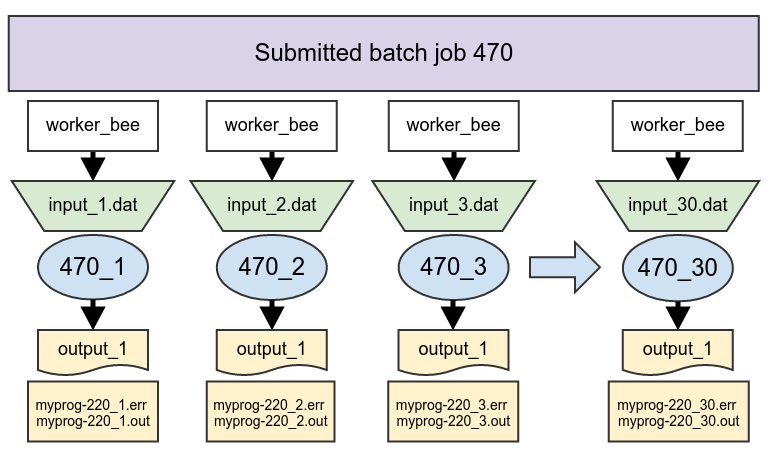
\includegraphics[width=0.90\textwidth]{images/job_array}
\end{center}
\end{frame}


\subsection{Batch Job Example Script Using Job Array}
\begin{frame}[fragile]
\frametitle{SLURM sbatch -- Submission Script File (Job Array)}
\begin{semiverbatim}\tiny
[login lus]\$ cat job_array.slurm

\#!/bin/bash
\#SBATCH \ddash{}job-name=example
\#SBATCH \ddash{}partition=community.q
\#\# 3 day max run time for community.q, kill.q, exclusive.q, and htc.q.  1 Hour max run time for sb.q
\#SBATCH \ddash{}time=3-00:00:00 ## time format is DD-HH:MM:SS
\#\# task-per-node x cpus-per-task should not typically exceed core count on an individual node 
\#SBATCH \ddash{}nodes=1
\#SBATCH \ddash{}tasks-per-node=1
\#SBATCH \ddash{}cpus-per-task=5
\#SBATCH \ddash{}mem=11000 \#\# max amount of memory per node you require
\textcolor{blue}{\#SBATCH \ddash{}error=myprog-\%A\_\%a.err} \#\# \%A - filled with jobid. \%a - filled with job arrayid
\textcolor{blue}{\#SBATCH \ddash{}output=myprog-\%A\_\%a.out} \#\# \%A - filled with jobid. \%a - filled with job arrayid
\#\# Useful for remote notification
\#SBATCH \ddash{}mail-type=BEGIN,END,FAIL,REQUEUE,TIME\_LIMIT\_80
\#SBATCH \ddash{}mail-user=user@test.org

source \ctilde/.bash_profile \#if you want to use modules or need environment variables, source your bash profile

\#\# All options and environment variables found on schedMD site: \href{http://slurm.schedmd.com/sbatch.html}{http://slurm.schedmd.com/sbatch.html}

export OMP\_NUM\_THREADS=\$\{SLURM\_CPUS\_PER\_TASK\}

./worker\_bee -i input\_\$\{SLURM_ARRAY_TASK_ID\}.dat -o output\_\$\{SLURM_ARRAY_TASK_ID\}
\end{semiverbatim}
\end{frame}



\subsection{Executing and Monitoring Job Array Batch Jobs}

\begin{frame}[fragile]
\frametitle{SLURM sbatch -- Executing \& Monitoring Job Arrays}\footnotesize
\begin{block}{Example}
\begin{semiverbatim}\tiny
[login lus]\$ sinfo
PARTITION     AVAIL  TIMELIMIT  NODES  STATE NODELIST
community.q   up     3-00:00:00 2      idle  compute-[0001-0002]

[login lus]\$ sbatch {\ddash}array=1-30 job_array.slurm
sbatch: Submitted batch job 470

[login lus]\$ squeue
JOBID      PARTITION    NAME     USER    ST   TIME    NODES  NODELIST(REASON)
470[3-30]  community.q  example  user99  PD   00:00   1      (resource)
470_1      community.q  example  user99  R    00:01   1      compute-0001
470_2      community.q  example  user99  R    00:05   1      compute-0002
\end{semiverbatim}
\end{block}
\end{frame}
